\documentclass[10pt]{report}

% PACKAGES
\usepackage[usenames]{color}
\usepackage{graphicx}

\newcommand{\mail}{\mailto{markus.mottl@gmail.com}}
\newcommand{\athome}[2]{\ahref{http://www.ocaml.info/#1}{#2}}
\newcommand{\www}{\athome{}{Markus Mottl}}

% INCLUDE HEVEA SUPPORT
\usepackage{hevea}

%BEGIN LATEX
\usepackage{natbib}
%END LATEX

\usepackage{amsmath}
\usepackage{amsfonts}
\usepackage{amssymb}
\usepackage{amsbsy}
\usepackage{accents}

\DeclareMathAlphabet{\mathsfsl}{OT1}{cmss}{m}{sl}

% HTML FOOTER
\htmlfoot{
  \rule{\linewidth}{1mm}
  Copyright \quad \copyright \quad 2009-
  \quad \www \quad \langle\mail\rangle
}

% HYPHENATION

\hyphenation{he-te-ro-ske-da-stic}
\hyphenation{ana-ly-ti-cally}
\hyphenation{know-ledge}

% TITLE

\begin{titlepage}

\title{\footahref{http://mmottl.github.io/gpr}{Gaussian Process Regression
with OCaml}\\Version 1.2.0}
\author{Markus Mottl\footnote{\mail}}

\date{\today}

\end{titlepage}

% DOCUMENT
\begin{document}

\maketitle

\begin{abstract}

This manual documents the implementation and use of the OCaml GPR
library for Gaussian Process Regression with OCaml.

\end{abstract}

\tableofcontents

\chapter{Overview}

The OCaml GPR library features implementations of many of the latest
developments in the currently heavily researched machine learning area of
Gaussian process regression.

\section{Background}

Gaussian processes define probability distributions over functions.
This allows us to apply probabilistic reasoning to problems where we are
dealing with \emph{latent functions}, i.e.\ functions that cannot be directly
observed or known with certainty.  By specifying prior knowledge about
these distributions in form of a \emph{mean} function and a \emph{covariance
function}\footnote{Sometimes also called a \emph{kernel}.} and making use of
Bayes' theorem, Gaussian processes provide us with a rigorous nonparametric
way of computing posterior distributions over latent functions given data,
e.g.\ to solve regression problems\footnote{Gaussian processes can also be
used for classification purposes.  This is by itself a large research area,
which is not covered by this library.}.  As more data becomes available,
the Gaussian process framework learns an ever more accurate reflection of
the probability distribution of latent functions that probably generate the
observed data.\\

Due to their mathematically elegant nature, Gaussian processes allow for
analytically tractable calculation of the posterior mean and covariance
functions.  Though it is easy to formulate the required equations, GPs come at a
usually intractably high computational price for large problems.  Typically,
only problems of up to a few thousand samples can be solved within reasonable
time.  Efficient approximation methods have been developed in the recent past to
address this shortcoming, and this library makes heavy use of them.\\

Gaussian processes are true generalizations of e.g.\ linear regression, ARMA
processes, single-layer neural networks with an infinite number of hidden
units, and many other more widely known approaches and modeling techniques.
GPs are closely related to support vector (SVM) and other kernel machines, but
have features that may make them a more suitable choice in many situations.
For example they offer predictive variances, Bayesian model selection,
sampling from the posterior distribution, etc.\\

It would go beyond the scope of this library documentation to provide for a
detailed treatment of Gaussian processes.  Hence, readers unfamiliar with this
approach may want to consult online resources, of which there are plenty.  This
section presents an overview of recommended materials.

\subsection{Video tutorials}

Video tutorials are probably best suited for quickly developing an intuition and
basic formal background of Gaussian processes and perspectives for their
practical use.

\begin{itemize}

\item \emph{\footahref{http://videolectures.net/gpip06\_mackay\_gpb}{Gaussian
Process Basics}}: David MacKay's lecture given at the \emph{Gaussian Processes
in Practice Workshop} in 2006.  This one hour video tutorial uses numerous
graphical examples and animations to aid understanding of the basic principles
behind inference techniques based on Gaussian processes.

\item
\emph{\footahref{http://videolectures.net/epsrcws08\_rasmussen\_lgp}{Learning
with Gaussian Processes}}: a slightly longer, two hour video tutorial series
presented by Carl Edward Rasmussen at the Sheffield EPSRC Winter School 2008,
which goes into somewhat more detail.

\item
\emph{\footahref{http://videolectures.net/mlss07\_rasmussen\_bigp}{Bayesian
Inference and Gaussian Processes}}: readers interested in a fairly thorough,
from the ground up treatment of Bayesian inference techniques using Gaussian
processes may want to watch this five hour video tutorial series presented by
Carl Edward Rasmussen at the MLSS 2007 in T\"ubingen.

\end{itemize}

\subsection{Books and papers}

The following texts are intended for people who need a more formal treatment and
theory.  This is especially recommended if one wants to be able to implement
Gaussian processes and their approximations efficiently, and build up the
background knowledge necessary for quick comprehension of publications in the
field.

\begin{itemize}

\item
\emph{\footahref{http://www.gatsby.ucl.ac.uk/\home{snelson}/thesis.pdf}{Flexible
and efficient Gaussian process models for machine learning}}: Edward Lloyd
Snelson's PhD thesis \cite{SnelsonThesis} offers a particularly readable
treatment of modern inference and approximation techniques for Gaussian
processes that avoids heavy formalism in favor of intuitive notation and
clearly presented high-level concepts without sacrificing detail needed
for implementation.  This library owes a lot to his work.

\item \emph{\footahref{http://www.gaussianprocess.org/gpml}{Gaussian Processes
for Machine Learning}}: many researchers in this area would call this book
\cite{oai:eprints.pascal-network.org:1211}, which was written by Carl Edward
Rasmussen and Christopher K.\ I.\ Williams, the ``bible of Gaussian processes''.
It presents a rigorous treatment of the underlying theory for both regression
and classification problems, and more general aspects like properties of
covariance functions, etc.  The authors have kindly made the full text and
Matlab sources available online.  Their
\footahref{http://www.gaussianprocess.org}{Gaussian process website} also lists
a great wealth of other resources valuable for both researchers and
practitioners.

\item \emph{Pattern Recognition and Machine Learning}: this book
\cite{BishopMachLearn} by Christopher M.\ Bishop thoroughly introduces the
reader to the field of machine learning, especially to Bayesian methods,
including Gaussian processes.

\item \emph{Matrix Analysis and Applied Linear Algebra}: readers who would like
to obtain a deeper understanding of the methods from linear algebra (e.g.\
matrix factorizations) used in the OCaml GPR library may find a most comprehensive and
detailed treatment in this book \cite{MatrixAnalysis} by Carl D.\ Meyer.

\end{itemize}

References to research about specific techniques used in OCaml GPR are provided
in the bibliography.

\section{Features of OCaml GPR}

Among other features the OCaml GPR library currently offers:

\begin{itemize}

\item Sparse Gaussian processes using the FI(T)C\footnote{\emph{Fully
Independent (Training) Conditional}} approximations for computationally
tractable learning (see \cite{conf/nips/2005}, \cite{SnelsonThesis}).  Unlike
some other approximations that lead to degeneracy, FI(T)C maintains sane
posterior variances, at almost no extra computational cost.

\item Safe and convenient API for computing posterior means, variances,
covariances, log evidence, for sampling from the posterior distribution,
calculating statistics of the quality of fit, etc.  The OCaml type and module
system as used by the API make sure that many easily made programming errors can
be avoided and guide the user to make efficient use of the library.

\item Optimization of hyper parameters via evidence maximization\footnote{Also
known as type II maximum likelihood.} including optimization of inducing inputs
(SPGP algorithm\footnote{This library exploits sparse matrix operations to
achieve optimum big-O complexity when learning inducing inputs with the SPGP
algorithm, but also for multiscales and other hyper parameters that imply sparse
derivative matrices for the marginal log likelihood.}).  The limited memory
BFGS2 algorithm in the \footahref{http://www.gnu.org/software/gsl}{GNU
scientific library} is employed for this purpose.

\item Supervised dimensionality reduction and improved predictions
under heteroskedastic noise conditions (see \cite{conf/uai/SnelsonG06},
\cite{SnelsonThesis}).

\item Sparse multiscale Gaussian process regression (see
\cite{conf/icml/WalderKS08}).

\item Variational improvements to the approximate posterior distribution (see
\cite{Titsias2009}).

\item Numerically stable GP calculations using QR-factorization to avoid the
more commonly used and numerically unstable solution of normal equations via
Cholesky factorization (see \cite{Foster2009}).

\item Consistent use of bindings to BLAS/LAPACK and C-code throughout key
computational parts of the library for optimum performance and conciseness.

\item Functors for plugging arbitrary covariance functions into the framework.
There is no constraint on the type of covariance functions, i.e.\ also string
inputs, graph inputs, etc., could potentially be used with ease given suitable
covariance functions\footnote{The library is currently only distributed with
covariance functions that operate on multivariate numerical inputs.  Interested
readers may feel free to contribute others.}.

\item Rigorous test suite for checking user-provided derivatives of covariance
functions, which are usually quite hard to implement correctly, and self-test
code to verify derivatives of marginal log likelihood functions using finite
differences.

\end{itemize}

\chapter{Using the library}

\section{Interface documentation}

The most important file for understanding the API is called \verb=Interfaces.ml=
and contained in the \verb=lib= directory.  It is already heavily documented so
we will only provide for a high-level view here.  Please refer to the OCaml file
for details.  Besides defining a few types, e.g.\ representations for sparse
matrices that users will have to use when communicating covariance matrices to
the system, the interfaces file contains two important submodules:

\begin{itemize}
\item \verb=Specs=, which contains signatures that users need to provide for
specifying covariance functions:
\begin{itemize}
\item \verb=Kernel=, the signature for accessing the datastructure that
determines a covariance function (= kernel) and its parameters.
\item \verb=Eval=, the signature of modules users have to implement to evaluate
covariance functions:

\begin{itemize}
\item \verb=Kernel=, a module satisfying the \verb=Kernel= signature above.
\item \verb=Inducing=, for evaluating covariances among inducing points.
\item \verb=Input=, for evaluating covariances involving single input points and
inducing inputs.
\item \verb=Inputs=, for evaluating covariances involving multiple input
points\footnote{Required separately besides evaluation of single inputs to force
the user to think about how to optimize for this case, which is quite
important.} and inducing inputs.
\end{itemize}

\item \verb=Deriv=, the signature of modules users have to implement to compute
derivatives of covariance functions:
\begin{itemize}
\item \verb=Eval=, a module satisfying the \verb=Eval= signature above.
Derivative code without the ability to evaluate functions would be rather
useless.
\item \verb=Hyper=, a module specifying the type of hyper parameters, for which
derivatives can be computed.
\item \verb=Inducing= and \verb=Input=, which provide a similar abstraction for
derivatives as the modules of same name provide for evaluation functions in
\verb=Eval=.  Note that computations between covariance evaluations and
derivatives can be shared.  This is especially useful and efficient for
covariance functions that use the exponential function.
\end{itemize}
\end{itemize}
\item \verb=Sigs=, which contains signatures a Gaussian process framework will
provide once it has been instantiated with a given covariance specification:
\begin{itemize}
\item \verb=Eval=, which contains modules the user can access to perform
computations in the Gaussian process framework:
\begin{itemize}
\item \verb=Spec=, the user-provided specification of the covariance function as
mentioned further above.
\item \verb=Inducing=, which contains functions to select and evaluate inducing
inputs.
\item \verb=Input=, for dealing with single inputs.
\item \verb=Inputs=, for dealing with multiple inputs.
\item \verb=Model=, for dealing with models.  A model is specified by the inputs
it consists of and the noise level.
\item \verb=Trained=, for dealing with trained models.  A trained model is a
model that has been trained on a given target vector.
\item \verb=Stats=, for computing statistics of the trained model (quality of
fit, etc.).
\item \verb=Mean_predictor=, minimalist datastructure for making mean
predictions.
\item \verb=Mean=, a posterior mean for a single point.
\item \verb=Means=, multiple means.
\item \verb=Co_variance_predictor=, minimalist datastructure for making
(co-)variance predictions.
\item \verb=Variance=, a posterior variance for a single point.
\item \verb=Variances=, multiple posterior variances.
\item \verb=Covariances=, posterior covariances.
\item \verb=Sampler=, sampling at a single point.
\item \verb=Cov_sampler=, sampling at multiple points (accounting for their
covariance).
\end{itemize}
\item \verb=Deriv=, which contains modules the user can access to perform
derivative computations for marginal log likelihoods within the Gaussian process
framework:
\begin{itemize}
\item \verb=Eval=, module satisfying the \verb=Eval= signature mentioned above.
\item \verb=Deriv=, module containing all the derivative code:
\begin{itemize}
\item \verb=Spec=, the user specification for covariance function derivatives.
\item \verb=Inducing=, \verb=Inputs=, \verb=Model=, \verb=Trained=, basically
mirror the role of the modules of same name in the \verb=Eval= signature.
\item \verb=Test= contains functions for testing both derivative code supplied
by the user and internal code using finite differences.
\item \verb=Optim= contains submodules for optimizing Gaussian processes,
currently only the \verb=Gsl= submodule, which uses the GNU scientific library
for that purpose.
\end{itemize}
\end{itemize}
\end{itemize}
\end{itemize}

\section{Predefined covariance functions}

The following modules implementing covariance functions already come with the
library:

\begin{itemize}
\item \verb=Cov_const=: the covariance of a constant function.
\item \verb=Cov_lin_one=: the covariance of a linear function with a single
hyper parameter (bias).
\item \verb=Cov_lin_ard=: the covariance of a linear function with
\emph{Automatic Relevance Determination} (ARD).
\item \verb=Cov_se_iso=: isotropic squared exponential covariance with amplitude
and length scale hyper parameters.
\item \verb=Cov_se_fat=: a highly parameterizable (``fat'') squared exponential
covariance function with amplitude, dimensionality reduction, multiscales, and
heteroskedastic noise support.
\end{itemize}

\chapter{Example applications}

There are currently three applications that are part of the distribution, two
for testing the library, and one simple command-line tool for solving regression
problems presented in comma-separated (CSV) files.

\section{Test applications}

The directory \verb=test= contains two applications.

\subsection{Derivative testing}

The application \verb=test_derivatives.native= generates random data to
run the internal test suite for checking the correctness of derivatives of
the marginal log likelihood function for the ``fat'' squared exponential
covariance function.  It prints out the hyper parameters it is currently
testing and would fail with an appropriate message if there were a problem.

\subsection{Test case for learning}

The application \verb=save_data.native= evaluates random inputs on some
known, nonlinear, one-dimensional function, adds noise, and then trains
a Gaussian process to learn the function from the data.  The application
writes out a number of results that can subsequently be visualized using
\footahref{http://www.r-project.org}{R} and cross-verified with a simple
\footahref{http://www.gnu.org/software/octave}{Octave} script.\\

Just run \verb=save_data.native=.  It will print out progress information
while performing evidence maximization to find suitable hyper parameters
and locations for inducing inputs.  This will not usually take more than a
few seconds (often just a fraction) unless the randomly chosen initial state
leads to a bad local optimum that is surrounded by an almost flat surface.
Just restart the run in this unlikely case.  Gaussian processes do not seem
overly prone to overfitting, but depending on the problem and the chosen
covariance function, evidence maximization may become trapped in local
optima. These local optima can be interpreted as alternative solutions if
they fit about equally well though. Once the application finishes, it will
store results in the \verb=test/data= subdirectory.

\subsubsection{Visualisation of results}

We can now execute \verb=R= on the command-line to run the visualization script
for this data by typing:

\begin{verbatim}
  source('display.R')
\end{verbatim}

This will visualize the data points, true mean and true confidence intervals,
the inferred mean function and its confidence intervals, samples of candidate
latent functions from the posterior distribution, locations of inducing inputs,
etc.  Here is an example:

\begin{center}
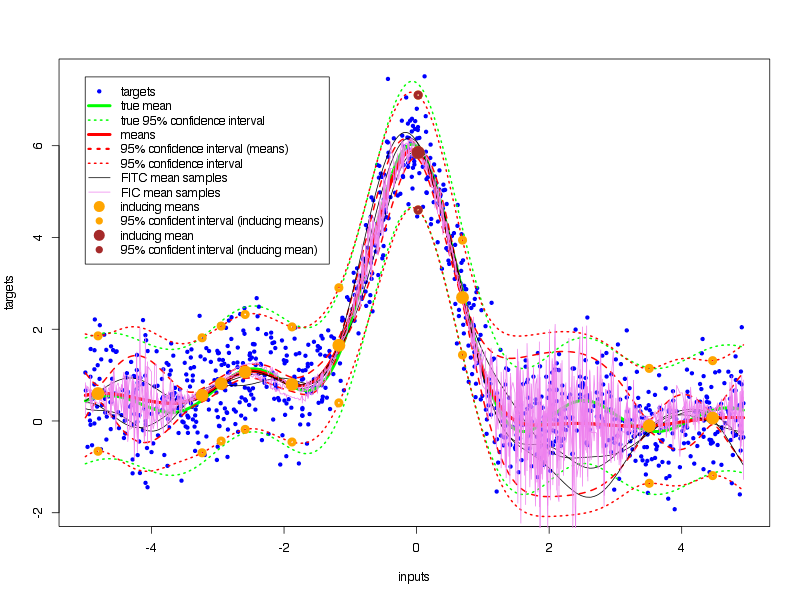
\includegraphics[width=12cm]{fit.png}
\end{center}

\subsubsection{Verification against Octave implementation}

There is also a small test suite for comparing results of
the OCaml library to equations written in Octave.  It, too,
depends on the data saved above by \verb=save_data.native=.
The Octave test suite does not use particularly efficient ways of
computing its results, but is fairly simple and readable.  It calls
\footahref{http://www.gatsby.ucl.ac.uk/\home{}snelson/SPGP\_dist.tgz}{Edward
Snelson's SPGP implementation} for reference.  The user may want to compile
the more efficient \verb=dist.c= file from within Octave first:

\begin{verbatim}
  mex dist.c
\end{verbatim}

\noindent Then source the test suite:

\begin{verbatim}
  source "oct.m"
\end{verbatim}

\section{Command-line tool}

The application \verb=ocaml_gpr.native= employs the OCaml GPR library
for implementing a simple utility to train and evaluate Gaussian process
models using the ``fat'' squared exponential covariance function and the
variational improvement \cite{Titsias2009} for model selection.  It reads
comma-separated values from standard input for both training and testing.
This application is considered to be an example only, but will likely be
extended in the future for more serious usage.\\

Datasets for regression problems that one may want to try out for testing can be
downloaded from many sites, one of the most well-known being the
\footahref{http://archive.ics.uci.edu/ml/index.html}{UCI Machine Learning
Repository}.

\subsection{Training models}

Here is an example invocation:

\begin{verbatim}
  ocaml_gpr.native -verbose -cmd train -model foo.model < data.csv
\end{verbatim}

It is assumed that the file \verb=data.csv= is comma-separated and that the last
column contains the target values.  The trained model will be stored in file
\verb=foo.model=.  It is generally recommended to use the \verb=-verbose= flag
for training, which will display various statistics at most once a second during
training iterations on standard error, e.g.:

{\footnotesize
\begin{verbatim}
  target variance: 84.41956
  iter    1: MSLL=18.9074776 SMSE=0.3878503 MAD=3.8968803 MAXAD=32.1662739
  iter    1: |gradient|=29911.88895
  iter  171: MSLL=-0.8875856 SMSE=0.2672445 MAD=2.9789019 MAXAD=34.0733409
  iter  171: |gradient|=57.08112
\end{verbatim}
}

The user can interrupt training at any time by pressing \verb=CTRL-C= if the
result seems good enough.  The best model found so far, as determined by the
mean standardized log loss (MSLL), will then be saved to the specified model
file.  It is also possible to specify a maximum number of iterations using the
flag \verb=-max-iter=.  Otherwise the optimizer parameters (see below) determine
when learning stops.\\

\subsubsection{Training flags}

Various flags can be passed to parameterize the learning process:

\begin{itemize}
\item \verb=-n-inducing= sets the number of inducing inputs.  The more points
are used, the more flexible the function that can be learnt.  Note that using as
many inducing points as there are inputs will not necessarily yield the full
Gaussian process, because the used approximation methods may also model
heteroskedastic noise.  Furthermore, the computational effort increases as
$O(M^3)$, $M$ being the number of inducing inputs.  The number of inducing
inputs will by itself not lead to overlearning, i.e.\ more is usually rather
better than worse. But increasing this number may lead to a larger number of
local optima and hence not necessarily better results.
\item \verb=-sigma2= sets the initial noise level hyper parameter.
\item \verb=-amplitude= sets the initial amplitude hyper parameter.
\item \verb=-dim-red= allows setting the target dimension for dimensionality
reduction of the input data.  None will be performed otherwise.  Note that one
can also specify the full dimensionality of the original input data, in which
case it will be subject to a fully general linear transformation, which will be
learnt in a supervised way in order to reveal useful features.
\item \verb=-log-het-sked= turns on support for improved learning of
heteroskedastic noise and sets the initial value for the logarithm of the
associated hyper parameters.  Negative values may often be required to avoid
getting trapped in bad optima right at the start.
\item \verb=-multiscale= turns on learning of multiscale parameters.
\item \verb=-tol=, \verb=-step=, and \verb=-eps= set the line search tolerance,
the initial step size, and the stopping criterion (gradient norm) for the
GSL-optimizer respectively.
\end{itemize}

It usually requires some experimentation to find out what kinds of parameters
may be most suitable for a given problem.

\subsection{Applying models}

Here is an example on how to apply models to test sets:

\begin{verbatim}
  ocaml_gpr.native -cmd test -model foo.model < test.csv
\end{verbatim}

It is assumed that the test set only contains inputs in its columns.  The mean
predictions for each input will be printed in the same order to standard
output.\\

By specifying \verb=-with-stddev= on the command line, a second column will be
printed separated by a comma, which contains the uncertainty of this mean
prediction expressed as a standard deviation.  If the flag \verb=-predictive= is
used, the noise will be included to yield a predictive distribution.

\chapter{Future work}

Besides improving the usability of the example application, a few extensions to
the library are considered for the near future:

\begin{itemize}
\item More flexible covariance functions.  Besides adding more such functions
and more features to e.g.\ the ``fat'' squared exponential covariance function
and making parameterization simpler, a very interesting approach would be to
support combining covariance functions.  As described in
\cite{oai:eprints.pascal-network.org:1211}, the sum and product of these are
also covariance functions, which would hence allow making better use of
problem-specific background knowledge.
\item Warping (see \cite{conf/nips/SnelsonRG03}) for nonlinear, nonparametric
transformations of the target variable.
\item Sparse convolved GPs (see \cite{DBLP:conf/nips/AlvarezL08}), which would
support multiple nonlinearly correlated target variables.  This would require
implementing the PI(T)C\footnote{\emph{Partially Independent (Training)
Conditional}} approximation (see \cite{SnelsonThesis}), which may also be
beneficial for solving particular problems.
\item Initialisation of inducing inputs using partial Cholesky factorization
instead of randomly chosen points.  This may be especially useful in the future
for problems that have non-numerical inputs, because these cannot be optimized
with numerical and even less so with efficient gradient-based methods.
\item A global optimisation framework that uses Gaussian processes to model loss
functions that are expensive to evaluate would seem like a great application to
add.
\end{itemize}

The interested reader may feel free to contribute these or other features.

\appendix

\chapter{Implementation details}

\newcommand{\red}{\textcolor{red}}
\newcommand{\blue}{\textcolor{blue}}

\newcommand{\dif}{\mathrm{d}}

\newcommand{\myu}[1]{\underaccent{\bar}{#1}}

\newcommand{\onehalf}{\tfrac{1}{2}}

\newcommand{\mat}[1]{\mbox{$\mathsfsl{#1}$}}
\newcommand{\myvec}[1]{\mbox{\boldmath$#1$}}

\newcommand{\diagv}[1]{\mathrm{diag_v}(#1)}
\newcommand{\diagm}[1]{\mathrm{diag_m}(#1)}
\newcommand{\trace}[1]{\mathrm{tr}(#1)}
\newcommand{\transv}[1]{\myvec{#1}^\top}
\newcommand{\transm}[1]{\mat{#1}^\top}

\newcommand{\imat}[1]{\mat{#1^{-1}}}
\newcommand{\itransm}[1]{\mat{#1^{-\top}}}
\newcommand{\chol}[1]{\mat{#1^{\onehalf}}}
\newcommand{\cholt}[1]{\mat{#1^{\tfrac{\top}{2}}}}
\newcommand{\ichol}[1]{\mat{#1^{-\onehalf}}}
\newcommand{\icholt}[1]{\mat{#1^{-\tfrac{\top}{2}}}}

\newcommand{\Km}{\mat{K_M}}
\newcommand{\iKm}{\imat{K_M}}
\newcommand{\dKm}{\mat{\dot{K}_M}}
\newcommand{\dKn}{\mat{\dot{K}_N}}
\newcommand{\Knm}{\mat{K_{NM}}}
\newcommand{\Kmn}{\transm{K_{NM}}}
\newcommand{\uKnm}{\myu{\mat{K}}_{\mathsfsl{NM}}}
\newcommand{\uuKnm}{\myu{\myu{\mat{K}}}_{\mathsfsl{NM}}}
\newcommand{\dKnm}{\mat{\dot{K}_{NM}}}
\newcommand{\uKmn}{\myu{\mat{K}}_{\mathsfsl{NM}}^\top}

\newcommand{\dl}{\dot{l}}

\newcommand{\vecu}{\myvec{u}}
\newcommand{\vecr}{\myvec{r}}
\newcommand{\vecs}{\myvec{s}}
\newcommand{\vect}{\myvec{t}}
\newcommand{\vecw}{\myvec{w}}
\newcommand{\vecv}{\myvec{v}}
\newcommand{\vecvx}{\myvec{v}_1}
\newcommand{\vecvy}{\myvec{v}_2}
\newcommand{\vecy}{\myvec{y}}
\newcommand{\uvecy}{\myu{\vecy}}

\newcommand{\vecsdh}{\onehalf\myvec{\dot{s}}}
\newcommand{\vecis}{\myvec{s}^{-1}}
\newcommand{\veciss}{\myvec{s}^{-\onehalf}}

\newcommand{\matB}{\mat{B}}
\newcommand{\matI}{\mat{I}}
\newcommand{\matQ}{\mat{Q}}
\newcommand{\matQn}{\mat{\widetilde{Q}}}
\newcommand{\tmatQn}{\transm{\widetilde{Q}}}
\newcommand{\matR}{\mat{R}}
\newcommand{\matS}{\mat{S}}
\newcommand{\matT}{\mat{T}}
\newcommand{\matU}{\mat{U}}
\newcommand{\matUx}{\mat{U}_1}
\newcommand{\matUy}{\mat{U}_2}
\newcommand{\matV}{\mat{V}}
\newcommand{\matW}{\mat{W}}
\newcommand{\matWx}{\mat{W}_1}
\newcommand{\matX}{\mat{X}}
\newcommand{\matXx}{\mat{X}_1}
\newcommand{\matWy}{\mat{W}_2}
\newcommand{\matXy}{\mat{X}_2}

\newcommand{\Lam}{\mat{\Lambda}}
\newcommand{\Lamss}{\mat{\Lambda}_{\sigma^2}}
\newcommand{\Lamssi}{\imat{\Lambda_{\sigma^2}}}


This section consists of equations used for computing the FI(T)C predictive
distribution, and the log likelihood and its derivatives in the OCaml GPR
library.  The implementation factorizes the computations in this way for several
reasons: to minimize computation time and memory usage, and to improve numerical
stability by e.g.\ using QR factorization to avoid normal equations, and by
avoiding inverses whenever possible without great loss of
efficiency\footnote{Unfortunately, inverses and symmetric rank-k operations are
unavoidable in some cases to preserve optimum big-O complexity.}.  It otherwise
aims for ease of implementation, e.g.\ combining derivative terms to simplify
dealing with sparse matrices.\\

The presentation and notation here is somewhat similar to \cite{SnelsonThesis}.
Thus, interested readers are encouraged to first read his work, especially the
derivations in the appendix.  Our presentation deviates in minor ways, but
should hopefully still be fairly easy to compare.  The log likelihood
derivatives have been heavily restructured though.  The mathematical derivation
of this restructuring would be extremely tedious, hence only the final result is
presented.\\

Here are a few definitions:

\begin{itemize}

\item $\mathrm{diag_m}$ is the function that returns the matrix consisting of
only the diagonal of a given matrix.  $\mathrm{diag_v}$ returns the diagonal as
a vector.

\item $\otimes$ represents element-wise multiplication of vectors.  A vector
raised to a power means element-wise application of that power.

\item Parts in \red{red} represent terms used for Michalis K.\ Titsias'
variational improvement to the posterior marginal likelihood (see
\cite{Titsias2009}).

\item Parts in \blue{blue} provide for an alternative, more compact, direct and
hence more efficient way of computing some result if the required terms are
already available.

\end{itemize}

\begin{eqnarray*}
\matV & = & \Knm\icholt{K_M} \\
\mat{\widetilde{K}_N} & = & \matV \transm{V} \\
\Lam & = & \diagm{\mat{K_N} - \mat{\widetilde{K}_N}} \\
\Lamss & = & \Lam + \sigma^2 \matI \\
\\
\vecr & = & \diagv{\Lam} \\
\vecs & = & \diagv{\Lamss} \\
\\
\uKnm & = & \ichol{\Lamss} \Knm \\
\matQ \matR & = & {\uKnm\choose\cholt{K_M}} \hspace{5mm}
\textrm{(QR-factorization of $\uKnm$ stacked on $\cholt{K_M}$)} \\
\\
\matB & = & \Km + \uKmn\uKnm = \transm{R}\transm{Q} \mat{Q} \matR = \transm{R}\matR \\
\matQn & = & {\lfloor \matQ \rfloor\footnotemark}_{N} \longrightarrow \uKnm = \matQn \matR \\
\matS & = & \ichol{\Lamss}\matQn\itransm{R} \\
\\
l_1 & = & -\onehalf (\log|\matB| - \log|\Km| + \log|\Lamss| + N \log 2\pi) \red{+ -\onehalf\vecis \cdot \vecr} \\
\\
\uvecy & = & \veciss \otimes \vecy \\
\vect & = & \imat{R} \tmatQn \uvecy \\
\vecu & = & \uvecy - \matQn \tmatQn \uvecy \\
\\
l_2 & = & \blue{-\onehalf \vecu\cdot\uvecy} = -\onehalf(\|\uvecy\|^2 - \|\tmatQn \uvecy\|^2) \\
l & = & l_1 + l_2 \\
\\
\matT & = & \imat{K_M} - \imat{B} \\
\\
\mu_* & = & \mat{K_{*M}} \vect \\
\sigma^2_* & = & K_* - \mat{K_{*M}}\matT\transm{K_{*M}} + \sigma^2 \matI \\
\end{eqnarray*}
\footnotetext{Take first $N$ rows.}

\begin{eqnarray*}
\matU & = & \mat{V} \ichol{K_M} \\
\\
\vecvx & = & \vecis \otimes (\vec{1} \red{\, + \, \vec{1} - \vecis \otimes \vecr} - \diagv{\matQn\tmatQn}) \\
\matUx & = & \diagm{\vecvx^{\onehalf}} \matU \\
\matWx & = & \matT - \matUx^\top\matUx \\
\matXx & = & \matS - \diagm{\vecvx}\matU \\
\dl_1 & = & -\onehalf(\vecvx \cdot \diagv{\dKn} - \trace{\transm{W}_1\dKm}) - \trace{\transm{X}_1\dKnm} \\
\\
\vecw & = & \veciss \otimes \vecu \\
\vecvy & = & \vecw \otimes \vecw \\
\matUy & = & \diagm{\vecw} \matU \\
\matWy & = & \vect \vect^\top - \matUy^\top\matUy \\
\matXy & = & \vecw\vect^\top - \diagm{\vecvy}\matU \\
\dl_2 & = & \onehalf(\vecvy \cdot \diagv{\dKn} - \trace{\transm{W}_2\dKm}) + \trace{\transm{X}_2\dKnm} \\
\\
\dl & = & \dl_1 + \dl_2 \\
\\
\tfrac{\partial l_1}{\partial\sigma^2} & = & -\onehalf(\mathrm{sum}(\vecvx) \red{\, - \, \mathrm{sum}(\vecis)}) \\
\tfrac{\partial l_2}{\partial\sigma^2} & = & \onehalf\mathrm{sum}(\vecvy) \\
\tfrac{\partial l}{\partial\sigma^2} & = & \tfrac{\partial l_1}{\partial\sigma^2} + \tfrac{\partial l_2}{\partial\sigma^2}
\end{eqnarray*}
\blue{
\begin{eqnarray*}
\vecv & = & \vecvx - \vecvy  \\
\matW & = & \matWx - \matWy = \matT - \vect \transv{t} - \matUx^\top\matUx + \matUy^\top\matUy \\
\matX & = & \matXx - \matXy = \matS - \vecw \transv{t} - \diagm{\vecv}\matU \\
\dl & = & -\onehalf(\vecv \cdot \diagv{\dKn} - \trace{\transm{W}\dKm}) - \trace{\transm{X}\dKnm} \\
\\
\tfrac{\partial l}{\partial\sigma^2} & = & -\onehalf(\mathrm{sum}(\vecv) \red{\, - \, \mathrm{sum}(\vecis)}) \\
\end{eqnarray*}
}

% BIBLIOGRAPHY
\bibliographystyle{alpha}
\bibliography{gpr_manual}

\end{document}
